\documentclass[sigconf]{acmart}

\renewcommand\footnotetextcopyrightpermission[1]{} % removes footnote with conference information in first column
\pagestyle{fancy} % removes running headers

\setlength{\parskip}{0pt}
\setlength{\parsep}{0pt}
\setlength{\headsep}{0pt}
\setlength{\topskip}{0pt}
\setlength{\topmargin}{0pt}
\setlength{\topsep}{0pt}
\setlength{\partopsep}{0pt}
%\linespread{0.95}
\usepackage{mdwlist}

\usepackage{amsmath}
\fancyhead{}
\settopmatter{printacmref=false, printfolios=false}
% Copyright
\setcopyright{none}
% \setcopyright{acmcopyright}
% \setcopyright{acmlicensed}
% \setcopyright{rightsretained}
% \setcopyright{usgov}
% \setcopyright{usgovmixed}
% \setcopyright{cagov}
% \setcopyright{cagovmixed}

\settopmatter{printacmref=false} % Removes citation information below abstract
\begin{document}
\title{Vector Semantics Evaluation}
\titlenote{https://github.com/feknall/vector-lexical-semantics}
\author{Hamid Fazli Khojir}
% \authornotemark[1]
\orcid{0000-0002-6033-6564}
\affiliation{
 \institution{University of Windsor}
%   \city{Fredericton} 
%   \state{NB} 
%   \country{Canada} 
}\email{fazlikh@uwindsor.ca}

\maketitle

\section{Introduction}
There are two different approaches for finding semantics of words, including lexical and vector mechanisms. Lexical semantics is a subfield of linguistic semantics that studies word meanings. The study includes how words structure their meaning, how they act in grammar, and the relationships between the distinct senses and uses of a word\cite{noauthor_lexical_2021}. We can consider it as a structured and supervised approach. On the other hand, vector semantic uses different mechanisms to find semantics of words without human supervision by converting each word or document to a vector of numbers.

\section{Motivation}
There are usually many different solutions for one problem. However, output of solutions are not always similar. Additionally, some solutions are more practical and scalable compared to other solutions. The main motivation behind our experiment is comparing two different vector semantics to see which one is has higher performance. Additionally, we can see that is it possible to reach to the golden model performance with these solutions or not.
\subsection{Motivating Example}
Similar words to 'old' based on lexical sentiment and SimLex dataset are: ['new', 'fresh', 'ancient', 'wide']. One of our word2vec models suggests ['when', 'around', 'This', 'guide', 'confront', 'see', 'arson', 'indicated', 'Negroes', 'Communists'] as close words to 'old'. Additionally, TF-iDF finds ['year', 'scriptures', 'possessive', 'paths', 'crossed', 'grads', 'mcn', 'miffed', 'basel', '39'] as close words. As we can see, lexical sentiment is really accurate compared to other approaches, but it needs human supervision.
\section{Problem Definition}
Given a golden standard $\mathcal{G}$ based on SimLex and two large corpuses of text $\mathcal{C}$ including news and romance genre of Brown corpus, calculate the average nDCG and Map of top-10 similar words retrieved by the vector semantics based on
TF-iDF and Word2Vec methods.
\section{Experiment}
\subsection{Datasets}
"SimLex" is our golden dataset, which has 1000 pairs of similarity between two words and a value that shows how much these two words are close to each other. Additionally, we have used news and romance genre of "Brown" dataset, which have 4623 and 4431 sentences, respectively. 
\subsection{Baselines}
If we consider the mechanism of vector semantics as a black-box, it gets a corpus of large texts as input, somehow it converts words of that corpus to a vector. After that, vectors that are close to each other can be considered as similar semantic. Cosine similarity is the most famous method to find the closeness of two vectors. 

For the Word2Vec mechanism, we trained 32 different models, which is combination of corpus: \{news, romance\}, context window size \{1, 2, 5, 10\}, and vector size \{10, 50, 100, 300\}, and we trained all of these models for 1000 epoch. We trained two different models for TF-iDF mechanism because of two different genres. 
\subsection{Results}
\begin{figure}[!htb]
\centerline{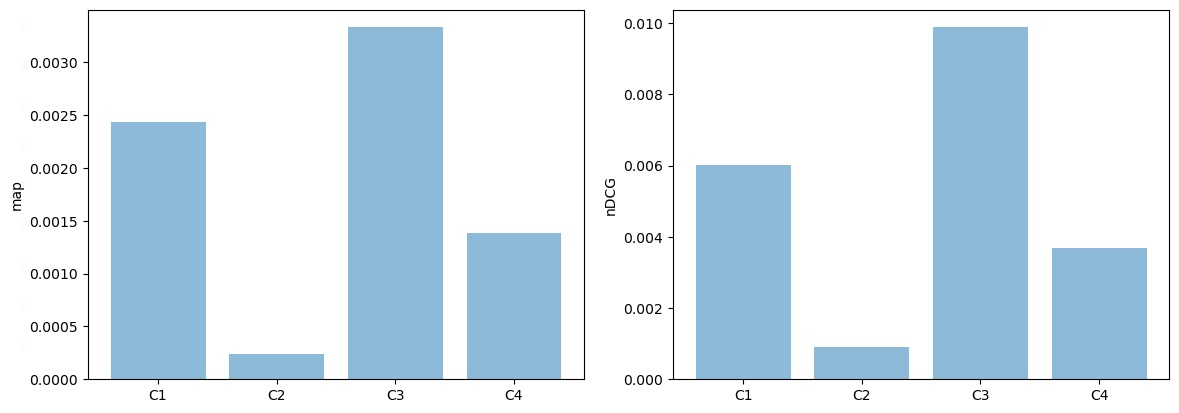
\includegraphics[width=22pc]{combined_horizontal.jpg}}
\caption{Comparison between Word2Vec and TF-iDF shows that Word2Vec has higher performance in both metrics}
\label{fig:ndcg}
\end{figure}
\begin{table}[!htb]
\begin{tabular}{ |c|c|c|c|c| } 
\hline
id & corpus & method & map & nDCG\\
\hline
C1 & news & Word2Vec & 0.002435 & 0.006004\\ 
C2 & news & TF-iDF & 0.000235 & 0.000917\\
C3 & romance & Word2Vec & 0.003331 & 0.009880\\
C4 & romance & TF-iDF & 0.0013868 & 0.003698\\
\hline
\end{tabular}
\caption{\label{tab:map-table}Performance of Word2Vec and TF-iDF according to map and nDCG metrics}
\end{table}
We report two different metrics, including nDCG and map. In both of these metrics, Word2Vec is multiple times better than TF-iDF. Additionally, we see that the corpus has key effect on the performance of vector semantics. For example, both Word2Vec and TF-iDF have higher performance when 'romance' genre is used instead of 'news'. 
\subsection{Findings}
Our results shows that vector semantics has a potential to capture lexical semantics. However, its performance is not comparable to lexical methods.
We see that word2vec is far better than TF-iDF in both nDCG and map metrics. However, word2vec needs a training time which makes it much slower than TF-iDF. By considering that training happens only once per setting, not per finding similarity, this downside can be ignored.

\bibliographystyle{ACM-Reference-Format}
\bibliography{bibliography.bib} 

\end{document}

